\section{Leads in the Labyrinth}
\margininbox{Slinging in the Rain}{
     \begin{itemize}
    \item Rhys Tyers
    \item Oliver Myerscough
    \end{itemize}}{\explo}
 
Despite much planning and scheming over the course of the year Oli and I had conspicuously managed to avoid caving with each other for most of the expo. With just a few days to go before derig we finally decided to put our plans into action. On a night train of course.
 
Oli and I were quick and slick down the entrance series. We caught up with Chris Keeley and co. just before camp. We overtook and geared up in the staging area in \passage{Friendship Gallery}. With an inappropriate feeling of optimism we packed the drill, gearing up for a big pitch series. Oli had spun wild tales of bottomless pitches and caverns measureless to man. Based on my previous experience of \passage{Yorkshire} and its continuations, I was doubtful. I found it hard to believe that the tight, thrutchy rift would develop into anything other than tight thrutchy rift but perhaps it would break into the master system and the mystery of \passage{Mig} would solved. 


 \begin{marginfigure}
\centering
\frame{\includegraphics[width=\linewidth]{"images/2013/rhys-sling-2013/rhys-skrbina".jpg}}
\label{Rhys Skrbina}
\caption{Rhys Tyers stands at the summit of \protect\passage{Vrh Nad \v{S}krbino} \pic{Dave Kirkpatrick}}
\end{marginfigure}

 
We snuck past the sleeping cavers in camp. Our gear clanked loudly and our swearing echoed as we climbed over the awkward mud wall beyond camp. Following \passage{Friendship Gallery} to the end, past the \passage[|see{Big Rock Candy Mountain}]{Big Rock} turning, brings you to a boulder strewn chamber. Somewhere here is a dug route downwards. It's long and sinuous and impresses upon you the lack of fear the Jana and co (the diggers) had. A couple of small chambers, and a big drippy pitch bring you to an immature streamway. Do not follow the water, climb above the water chamber (Tetley and I had followed the water previously down far too much grim immature stream, still a lead though). 
 
Then it's  just a matter of following the thrutchy vadose passage. Occasionally Oli led me into a dry meander that would then rejoin the streamway again. I don't think anyone has followed the stream all the way down, so who know's if there's anything off there. At some point there's an interesting climb down into the stream again where you cross over the rift and double back. There's also a small section with a quite a few dry passages heading off, supposedly thoroughly explored by Saber and Oli. 
 
Once at the limit of exploration Oli coaxed me forwards, to the head of the `bottomless' pitch. Gently I edged forwards until I could see down, all of perhaps 10 metres to the floor. Oli assures me that his previous claim was misremembering and not in fact a trick to lure me to his pet shit lead. Still, though not deep, the passage bellowed out into a middling sized chamber. \bignote{With a big bag full of equipment we barely knew how to use there was nothing to stop us}. Oli retrieved the drill, clipped in the drill bit, attached the battery and set to work tunneling a new home for our shiny raul bolts. 
 
Quite a while later, with no progress, and after several attempts at drilling in various spots  Oli told me what he thought the problem could be. Super hard rock? A blunt drill bit? Maybe he wasn't pushing the drill hard enough. I pondered. 

`You've got the drill in reverse' I offer. 





We swap places and with the drill rotating in the correct direction I try again. I successfully drill a hole and place a bolt but carelessly hammer it on so that the end deforms and I can't get the nut on. So much for that. Frustrated and itching to get down the pitch we scanned the surrounding rock. We located a nodule of rock sufficiently large to abseil off (but not too large as to make you overconfident in its abilities as an anchor, that too would be a mistake) and a second, further back in the passage. We gave each a fetching green nylon choker, attached our ropes and I headed down.
 
 
 \begin{marginfigure}
\centering
\frame{\includegraphics[width=\linewidth]{"images/2013/rhys-sling-2013/izi-monatip".jpg}}
\label{Monatip-rigging}
\caption{Rigging one of the new finds in Monatip \pic{Iztok Mo\v{z}ir}}
\end{marginfigure}

Unfortunately our carefully chosen anchors placed me perfectly under the small stream that we'd been following all the way from \passage{Yorkshire}. I scrambled desperately at the wall and clawed my way out of the water. I looked around. I wanted a nodule, flake, a stal, anything for a deviation. Smooth walls offered me nothing but glistening reflections. I was however gripping a small crack in the wall. I tied an overhand in both ends of a sling, rethreaded one (for a krab) and inserted the other end of the sling into the crack and pulled it, till the single overhand was wedged. I clipped the krab above me and carefully loaded my crack deviation. It held.



\begin{marginfigure}
\centering
\frame{\includegraphics[width=\linewidth]{"images/2013/rhys-sling-2013/jarvist_tetley_at_camp".jpg}}
\label{Monatip-rigging}
\caption{Tetley at underground camp \pic{Jarvist Frost}}
\end{marginfigure}

At the bottom it became apparent that we were just on a ledge. The ledge was flat and washed clean. A 5\,m by 5\,m by 15\,m deep hole was in front of us, large boulders perched precariously above it.  Across the holes, at the same height as the ledge was a crawl going off. To the right was a crack, filled with boulders, descending into the shaft. Up from the crack a small hole led off. A crawl can be seen heading off but looks a little immature. We headed back and began thinking about how to get down the pitch.
Oli decided it would be incredibly dangerous to attempt to descend the pitch without proper gardening first. I suspect he just wanted to push big boulders down the pitch. He pushed a couple, varying from the classic TV sized boulder to some approaching human size. They went down with a spectacular bang. He was right though, it didn't take much to push them down. He went for another one. I winced expecting the loud crash but nothing came. The two Oli sized boulder had become wedged on the edge of the lip and the far wall (there was a sort of corner with the crack). On the near side it was stuck on a tiny protrusion from the wall. I tried to hit it with a hammer but it was surprisingly solid. We looked at each other. There was no way we could descend with this death hanging above us. 
 
\bignote{Oli decided to solve this problem as he solves all his problems}. He started throwing rocks at the rock. Gradually the rock inched further downwards. Each thrown rock budging it down another few millimetres. Eventually it fell. It was a close thing to as we were running out of rocks to `garden' with.
 
We looked about for some good rock to bolt in but found none. Eventually we squeezed into the crack and found some suitable naturals to descend on. At the bottom we landed on what had been a clean flat floor, now littered with the remains of our gardening. The water trickled ahead into stooping passage and very quickly sumped. It was very pretty, all blue green against nice white rock but it wasn't what we were hoping for. We climbed back up.
 
Going up the crack there was a small passage. We crawled up this a way until it brought us out in a small chamber with some water trickling from 5 or so metres above us. It might be possible to free climb this but you'd probably want to bolt it. Back down again and we turned our eyes to the final lead, the crawl across the other side of the chamber.
 
We were hand bolting by this point having become frustrated with our ineptitude with the drill. 3 or 4 bolts brought us safely into the crawl. Down the sandy abandoned phreatic passage, we came to a point where two boulders blocked the way. We tried moving them but they wouldn't budge. 

\margininbox{Lead advice}{Beyond, the crawl continues, likely bypassing the perched sump. A bit of capping or even feather and wedging would get you past. \protect\mininame{Rhys Tyers}}{\logbook}
 
Back at camp we collapsed. I awoke 12 hours later and tried to cajole Oli into going pushing or maybe even heading out but he was not a man who could be moved. Another 10 hours passed.  We were alone, on the last pushing trip of the expo. We got up att 11\,pm or so, packed up as much as we could to get the f out of there. The next day everyone else would come down to haul the rest of the camp stuff out and the derigger would do the needful. The weather forecast predicted armageddon at 12\,am. As we packed we realised we could get everything into 5 bags, most of which would be relatively light. So we took 5 bags. Oli took the two heavy ones and I took the three light ones. Another 5 hours and we emerged into the morning light and drizzle. A few bleary faces greet us at the bivi.

\name{Rhys Tyers}

\begin{pagefigure}
\frame{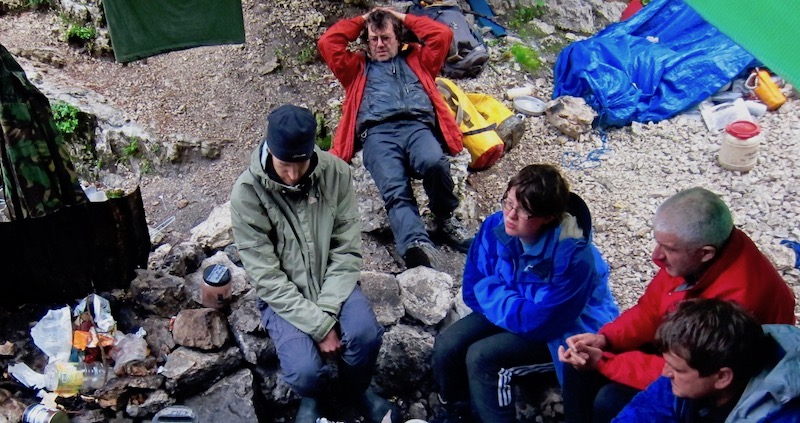
\includegraphics[width = \textwidth]{images/2013/rhys-sling-2013/kate_bivi_faces.jpg}}
\caption{A few bleary faces in the bivi greet returning explorers after a stormy night and relentless, cold burja winds blowing from the north \pic{Kate Smith}} \label{fig:bivi_bleary_faces}
\end{pagefigure}
